\chapter{Implementation of Constraint Generator}
I implemented fully automated certification platform for python source code  using two python scripts, given in Appendix \ref{ch:script1} and \ref{ch:script2}. Block diagram in figure \ref{fig:script1} shows modules of script1, first python source code is converted into abstract syntax tree (AST) with the help of ast library. The purpose of this step is to avoid tedious work of parsing of source code and comments. Figure \ref{fig:parsing} shows that parsing function reads AST word by word. If function finds any desired word it calls other handler functions to handle code related to particular word, for example: if "While" word is found, parsing function parses body of while and passes it as argument to while\_handler(while\_code) function. Handler function parses variables used in condition and passes the body part to parsing function again. Whenever parsing function finds assignment operation it generates constraint and goes to next word.     
\begin{figure}
	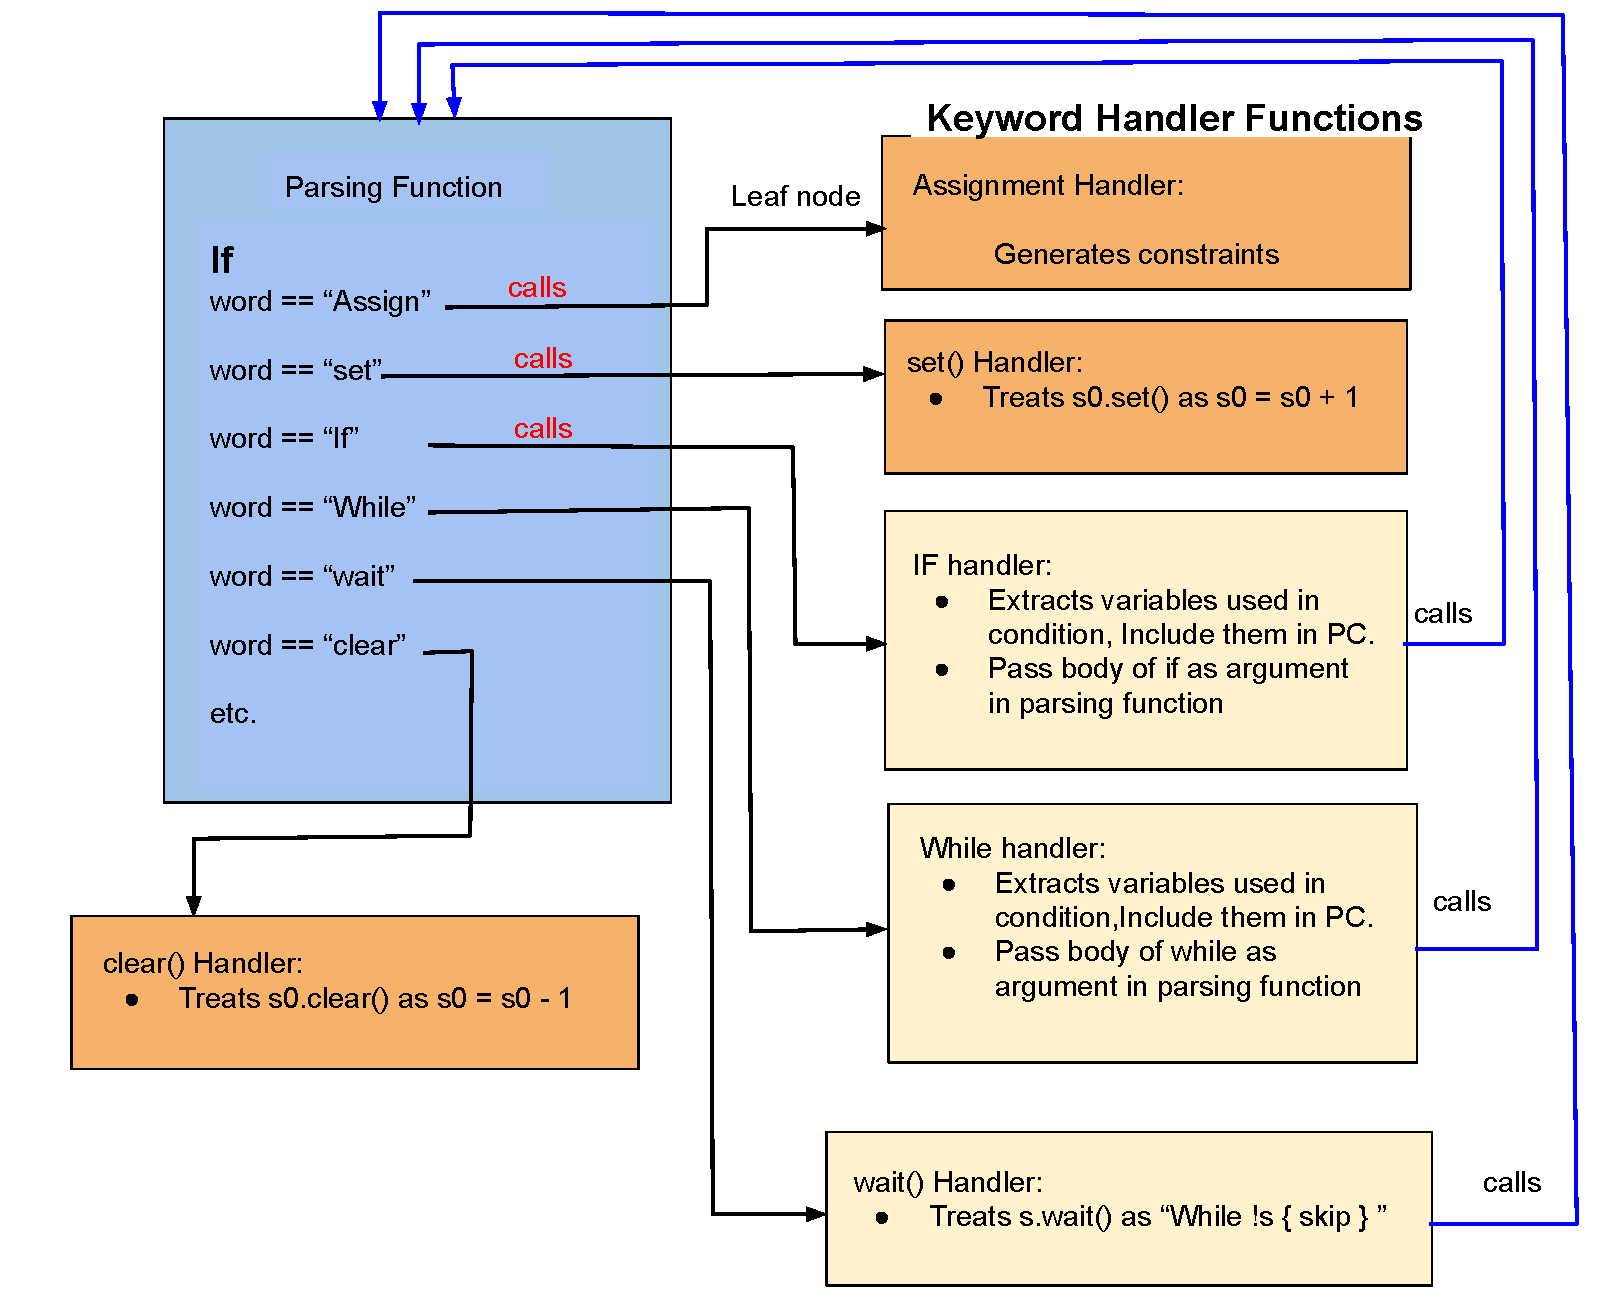
\includegraphics[width=1\textwidth]{parsing.pdf}
	\centering
	\caption{Block diagram of parsing function}
	\label{fig:parsing}
\end{figure}
	The Block diagram for script 2 is given in figure  of chapter . 
	Effectiveness of this platform depends on the phase of constraint generation because if constraint generator fails to track information flow properly then verifier can not produce correct results. Chapter \ref{ch:certify} describe about different constraint generators. Chapter  shows the comparison among all constraint generator.  